\documentclass{article}
\usepackage[preprint, nonatbib]{neurips_2019}

\usepackage[utf8]{inputenc} % allow utf-8 input
\usepackage[T1]{fontenc}    % use 8-bit T1 fonts
\usepackage{hyperref}       % hyperlinks
\usepackage{url}            % simple URL typesetting
\usepackage{booktabs}       % professional-quality tables
\usepackage{amsfonts}       % blackboard math symbols
\usepackage{nicefrac}       % compact symbols for 1/2, etc.
\usepackage{microtype}      % microtypography
\usepackage[authoryear,square,numbers]{natbib}
\usepackage{graphicx}
\usepackage{amsmath}
\bibliographystyle{abbrvnat}

\title{Kernel Bandwidth Selection via SGD}

\author{%
  Gilberto Garcia P\'{e}rez \\
  \texttt{gilberto.gape@gmail.com} \\
  % examples of more authors
  \And
  Andr\'{e}s Potapczynski\thanks{...} \\
  \texttt{ap3635@columbia.edu}
  % Address \\
  % \texttt{email} \\
}

\begin{document}

\maketitle

\begin{abstract}
  We propose an algorithm to select the kernel bandwidths that is faster when compare
  to the standards approaches and is scalable in the number of variables. The standard
  methods select the bandwidth by using derivative free optimization and rely
  on computing the generalization error based on LOO. This optimization technique does
  not scale to the number of variables and the generalization error based on LOO
  is highly biased. We circumvent both problems by posing an optimization problem
  that computes a better generalization error and that uses the gradient to efficiently
  explore the parameter space.

\end{abstract}

\section{Introduction}

\begin{itemize}
  \item Check exhaustively that the idea has not been developed elsewhere.
  \item Revise the kernel regression literature to see what it the most novel technique
  \item Expand Motivation from abstract.
  \item Explain how AD makes this idea possible and computationally feasible \citet{AD}
  \item Mention that the code is available in GitHub
\end{itemize}

\section{Mathematical Formulation}

The following idea has been explored in \citet{hyperopt} and can be applied to
any Machine Learning model easily. Let $\omega \in \Omega$ denote the $H$
hyperparameters of a given model. We reparameterize each $\omega_j$ as a function of $\xi_j$
for $j=1,\dots,H$ where $\xi \in \mathbb{R}^H$. Thus, we want to minimize

$$F(\xi)=L( y^{test}, \hat{y}(x^{test}, \xi, \mathfrak{D}^{train}) )$$

where $L(\cdot, \cdot)$ is a loss function that estimates the generalization error of the
model, $y^{test}$ is the test data being used for the estimation and $\hat{y}$ are the
predictions that depend on both the hyperparameter choice $\xi$ and the training data
$\mathfrak{D}^{train}$. Thus, we use AD to numerically compute

$$\nabla F(\xi) = \nabla L(y^{test}, \hat{y}(x^{test}, \xi, \mathfrak{D}^{train})) \nabla
\hat{y}(x^{test}, \xi, \mathfrak{D}^{train})$$

and hence enable an updating schema of the form

$$\xi^{t+1} = \xi^{t} - \rho \nabla F(\xi^{t})$$

where $t$ denotes the iteration number and $\rho$ the step-size. As implicitly stated above,
we need that $\nabla \hat{y}(\cdot, \cdot,\cdot)$ and $L(\cdot, \cdot)$ be differentiable
functions on the appropriate argument. The choice of $L(\cdot, \cdot)$ used in this paper is
the usual $M$-fold CV MSE estimator.

$$L(y^{test}, \hat{y}(\xi,\mathfrak{D}^{train})) =
\frac{1}{M}\sum_j^{M}\sum_i^{N_j}(y_i^{test_j} -
\hat{y}_i(x_i^{test_j}, \xi, \mathfrak{D}^{train_j}))^2$$

where $N_j$ denotes the number of test observations in fold $j$ for $j=1, \dots, M$,
$y_i^{test_j}$ is the $i$-th label/output for fold $j$, similarly $x_i^{test_j}$ is the
$i$-th test observation for fold $j$, $\mathfrak{D}^{train_j}$ the training data available
in fold $j$ and, finally, $\hat{y}_i(x_i^{test_j}, \xi, \mathfrak{D}^{train_j})$ is the
model's prediction. As illustration, we show the functional forms for the case of
Kernel Regression,

$$ \hat{y}_i(x_i^{test_j}, \xi, \mathfrak{D}^{train_j}) =
\sum_{r}^{N_j^{train}}
y_{r}^{train_j} \frac{K_h(x_i^{test_j} - x_{r}^{train_j})} {
\sum_k K_h(x_i^{test_j} - x_{k}^{train_j})} $$

where

$$
K_{h}(z) = \exp \left( - \frac{1}{2} \sum_d^{D} \left( \frac{z_d}{h_d} \right)^{2} \right)
$$

and the bandwidth is again re-parameterized positively as $h = \exp(\xi)$

\section{Experiments}

\subsection{Kernel Regression}

For our toy simulation, we used a function of two variables where having a different
bandwidth for each would be advantageous. For that, we set a linear dependence on the first
variable and a non-linear on the second. Moreover, we added interactions effects to increase
the difficulty of the problem. Therefore, after sampling $x_i^{(s)} \sim U[0, 10]^2$ and
$\epsilon_i^{(s)} \sim N(0,0.5)$ we generated
$$
y_i^{(s)} =
x_{i,0}^{(s)} - \left( x_{i,1}^{(s)} \right)^{2} + 0.3 \log \left(1 + x_{i,0}^{(s)} \cdot
x_{i,1}^{(s)} \right) + \epsilon_i^{(s)}
$$
for $i=1, \dots, N$ and $s=1, \dots, S$ where $N$ is the number of observations for each
sample and $S$ the total number of samples. In figure \ref{krr} we summarize the results.
Similar to the previous experiment, we see on the right plot that the error decreases
rapidly and almost at 20 iterations all the simulations have converged. Additionally, on the
plot of the right we exhibit the qualitative improvement that having two bandwidths creates
by having a much smoother approximation in the end of the range.

\begin{figure}
  \centering
  \caption{Kernel Regression Simulation Results.}
  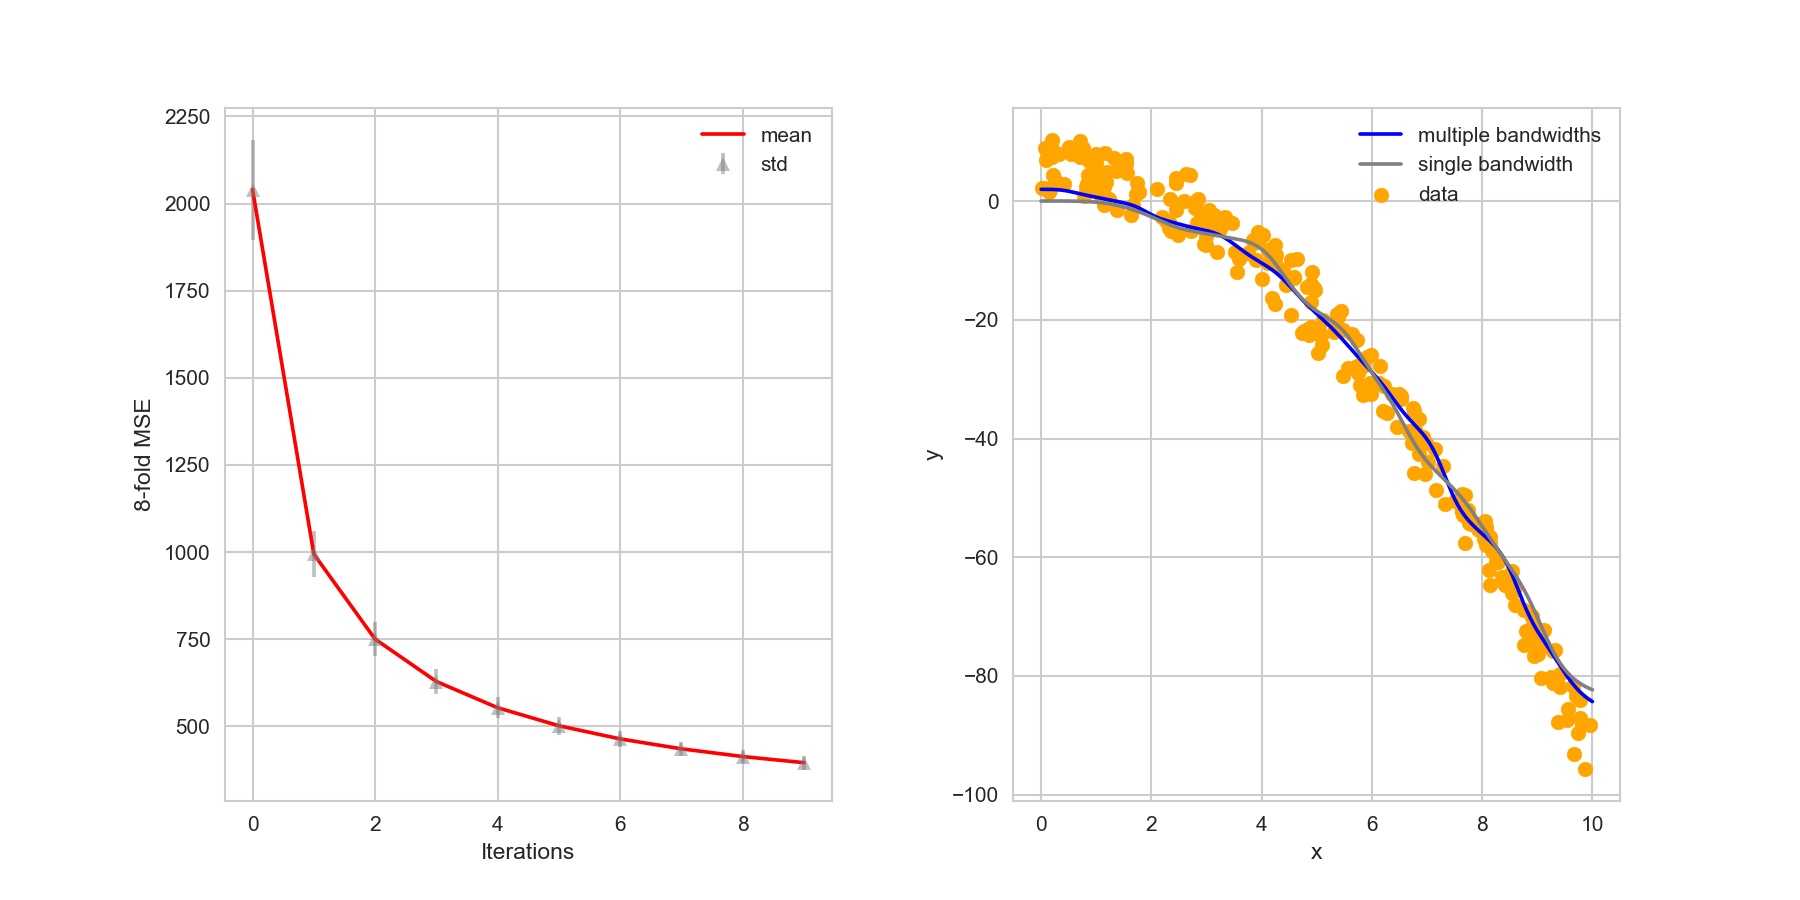
\includegraphics[width=\textwidth]{./pics/ker_reg_results.png}
  \label{krr}
\end{figure}

\begin{figure}
  \centering
  \caption{Kernel Regression Simulation Results.}
  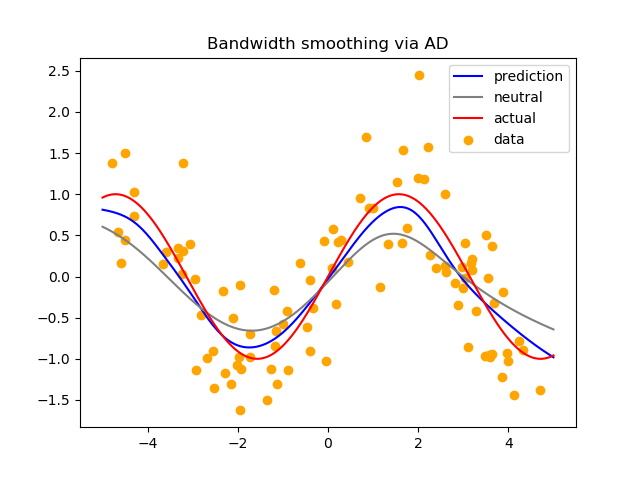
\includegraphics[width=\textwidth]{./pics/example01.png}
  \label{krr}
\end{figure}

As for the real-life data set example, we again used an example of \citet{ESL} but now from
its kernel Regression chapter. We used the South African Heart Disease data. \textbf{[...]}

\citet{ADAfaEPoV}


\section{Conclusions}

\textbf{[...]}

\section{Future Work}

\textbf{[...]}

\bibliography{SGD_ref}

\end{document}
